\section*{Anna Hyndr\'akov\'a}
Die Jüdin Anna Hyndr\'akov\'a\index{p}{Hyndr\'akov\'a, Anna} wurde 1928 in Prag\index{o}{Prag} geboren und verbrachte ihre gesamte Jugend, bis zu ihrer Deportation nach Teresienstadt (Terez\'in, Tschechien), in der tschechoslowakischen Hauptstadt. Zusammen mit ihrer Familie kam sie im Dezember 1943 zunächst nach Auschwitz-Birkenau und kurz darauf allein ins Groß-Rosener KZ-Außenlager Christianstadt (Krzystkowice, Polen). Während der Evakuierung des Lagers ergriff sie mit zwei jungen Tschechinnen (Eva Preissov\'a\index{p}{Preissov\'a, Eva} und Doris W.\footnote{Aussage von Doris W. JMP Kassette 099.}) die Flucht. Ohne Orientierung in der Fremde gelangten sie in die kleine Gemeinde Ödernitz\index{o}{Ödernitz} bei Niesky\index{o}{Niesky}. Ohne es zu wissen, erbaten sie auf einem Gehöft eines SS-Mannes Unterkunft und Nahrung. Dieser gewährte ihnen Einlass und Essen, doch meldete sie am darauffolgenden Tag den Wachleuten des KZ-Außenlagers Niesky\index{o}{Niesky} (Wiesengrund). Nach kurzem Aufenthalt im dortigen Männerlager wurden sie schon bald nach Görlitz verlegt. Der vorliegende Text in einer Übersetzung des Autors aus dem Englischen entstammt einer Publikation des Staatlichen Jüdischen Museums in Prag\index{o}{Prag}. Anna Hyndr\'akov\'a\index{p}{Hyndr\'akov\'a, Anna} selbst war Mitarbeiterin des Museums und veröffentlichte den Originaltext als Brief an ihre beiden Kinder (\glqq Letter to my Children\grqq\footnote{Anna Hyndr\'akov\'a: Letter to my Children. In: World without human dimension.}) in der tschechischen Samisdat Serie \glqq Petlice\grqq und gleichzeitig im Samisdat \glqq Středn\'i Evropa\grqq (Mitteleuropa).

\paragraph{Liebe Alena und lieber Pavel!}
Ich glaube ihr wisst alles oder fast alles über mich -- wie auch immer, in einem nachgiebigen Moment versprach ich euch einen Brief zu schreiben und dies versuche ich nun. Meine literarischen Ambitionen habe ich vor langer Zeit, bereits als Schulmädchen, aufgegeben. Es gab Zeiten da wollte ich eine Schriftstellerin sein und schrieb Schulaufsätze, nur um ein paar auf Lager vorrätig zu haben und mit ihnen zu handeln. Seht ihr? Mit diesen Worten habe ich in der Tat begonnen einen Brief zu schreiben. Es wäre mir schwer gefallen dies viel früher zu tun.[\dots]
Sie setzten uns auf einen Lastwagen, vertrauten uns der Obacht eines alten Schutzpolizisten an und wir fuhren fort ins Arbeitslager Görlitz. Dieses war ebenfalls eine Nebenstelle des Lagers in Groß-Rosen. Es bestand aus einem kleinen Frauenlager mit ungefähr 300 ungarischen Frauen mit rasierten Köpfen und einem großen Hauptlager der Männer. Wir wurden vom Lagerältesten, Herman Czech -- einem deutschen Kriminellen, Sadisten, von kleiner hässlicher Gestalt -- empfangen. Er hatte drei abgerichtete, schwarz-weiße Mastifs und war der Schrecken des ganzen Lagers, obwohl er selbst ein Gefangener war. Der Polizeimann, der uns ins Lager brachte, glaubte, es sei ein großer Scherz, als er sagte, dass wir von einem Transport geflohen seien. Für ihn erschien es, angesichts unseres Zustands, absurd und er dachte, es wäre sehr witzig. Unbefangen und korrekt nahm Czech dies ernst. Er nahm uns entgegen und entschied sofort über unsere Bestrafung: Köpfe rasieren und 25 Hiebe mit der Peitsche, die er für seine Hunde hatte. Wir glaubten, es wäre das Ende, wir würden die Folter womöglich nicht überleben. Sie fingen an, nach einer Bank, einem Barbier (es sollte ein öffentliches Ereignis werden) und jemanden, der die Schläge ausführt, zu suchen. Unsere Ankunft hatte Aufregung verursacht und niemand wollte uns Schaden zufügen, niemand beeilte sich. Wir standen und warteten, bis plötzlich ein Transport ankam, der das Görlitzer Lager während der Evakuierung ihrer eigenen beiden Lager passieren wollte. Es wurde sofort bekanntgegeben und Czech hatte sich darum zu kümmern. Unsere Bestrafung wurde verschoben und er brachte uns ins Frauenlager. Die Baracken dort waren anders als jene, die wir gewohnt waren. In der einen Hälfte waren die Schlafstätten, in der anderen Hälfte Tische und Bänke, die als Esszimmer dienten. Wir mussten vor einem Fenster stehen, so dass sie uns sehen konnten, und auf unsere Bestrafung warten. Niemandem war es gestattet, mit uns zu reden und wir durften uns nicht hinsetzen. Folglich standen wir da eine ganze Weile, aber der Abend kam, am folgenden Tag kam ein neuer Transport und dieses Schema wiederholte sich viele Tage lang. Langsam begannen wir uns in der Baracke zu bewegen. Wir konnten nicht nach draußen gehen, weil wir mit unseren langen Haaren zu auffällig waren. Es war unser großes Glück als ein Transport mit polnischen Frauen ankam -- da waren 300 von ihnen und sie hatten ebenfalls langes Haar. Wir wurden in der Menge ununterscheidbar in Bezug auf Erscheinungsbild und Sprache, die Deutschen waren nicht fähig, den Unterschied zwischen der polnischen und tschechischen Sprache herauszuhören. Bevor Czech uns bestrafen wollte, erhielt er auch den Befehl, das Lager zu evakuieren. In dem Durcheinander, das darauf folgte, hatte er uns vollkommen vergessen. Vermutlich half uns auch die Lagerälteste des Frauenlagers, eine Wiener\index{o}{Wien} Jüdin namens Stella, die sehr vernünftig und freundlich war. Sie empfand Zuneigung uns gegenüber; wir sprachen deutsch und hatte den selben kulturellen Hintergrund wie sie.

Auf einmal nahmen die Symptome von Doris' Tuberkulose bedenklich zu. Sie begann, Blut zu husten. Wir glaubten, dass wir beide Tuberkulose hätten, da wir die ganze Zeit zusammen verbrachten, und vor allem auch in derselben Baracke. Jedenfalls konnten wir erst einmal nichts tun, am Leben zu bleiben war immer noch das größere Problem als gesund zu sein. Trotzalledem fühlten wir uns ausgeruht genug, die vor uns stehenden Märsche ohne Furcht anzutreten. Außerdem war es nicht mehr so eisig kalt. Natürlich gingen wir zu Fuß, es gab nur wenige Wagen mit den Sachen der Deutschen und dem Proviant. Sie nannten uns \glqq Die drei Tschechen\grqq, seitens der anderen Gefangenen galt uns ein großes Interesse. Sie wussten von uns, doch hatten sie bis dahin noch keine Gelegenheit, mit uns Kontakt aufzunehmen. Sie wussten, dass wir in Auschwitz gewesen und geflohen waren. Die deutschen Gefangenen spürten eine engere Beziehung zu uns als zu den Ungarinnen oder Polinnen, da wir ihre Sprache sprachen und in der Lage waren, mit ihnen zu kommunizieren. Deshalb wunderten wir uns auch nicht über die Aufmerksamkeit, die uns ein Wagenkutscher -- ein deutscher Jude aus Köln\index{o}{Köln} mit dem Namen Samuel Kessler\index{p}{Kessler, Samuel}\footnote{Im englsichen Originaltext wurde der Name der Person seitens der Autorin absichtlich in \glqq Salamon Ressler \grqq~geändert. Interview mit Ana Hyndrakova, Prag 2005.} schenkte. Er war 33 Jahre alt und hatte seine Frau in Auschwitz verloren. Als Kutscher hatte er eine gute Position im Lager sowie auf dem Weg, und deshalb gab er uns Essen. Manchmal nahm er uns auch auf seinem Wagen mit, wenn sich die Marschkolonne übermäßg weit hinzog. Er gewann bald unser Vertrauen, seine Einstellung gegenüber uns war freundschaftlich und, so schien es mir, väterlich. Er war sehr freundlich. Als wir einmal die Nacht in einer großen Scheune verbrachten, suchte er für uns den besten Platz aus und brachte uns frisches Stroh. Schon bald schliefen wir alle ein und als ich wegnickte, spürte ich, wie er meine Füße mit seinem Mantel bedeckte. Etwas später wachte ich auf. Er streichelte mich und flüsterte mir zu, dass er mich will und auf mich achtgeben würde. Da habe ich bemerkt, dass sein Interesse nicht väterlich war. Ich brachte ihm nicht viel Widerstand entgegen, ich hatte weder die Kraft noch den Willen. Es schien mir, dass wer immer sich mir gegenüber nett verhielt, würde früher oder später mit mir schlafen wollen, so dass ich sowieso keinen Erfolg hätte, es abzuwehren. Es war wie eine Fortsetzung des Schreckens in Niesky. Von da an versuchte er bei jeder Gelegenheit, bei mir zu sein; manchmal konnte ich ihm entkommen, manchmal nicht. Ich war verzweifelt und blind. Ich habe nicht verstanden, dass er mich vielleicht wirklich liebt und sich nicht nur im Lager um mich kümmern würde, sondern auch nach dem Krieg. Mir schien es, als hätte er in mir jemanden gefunden, der den Platz seiner toten Frau einnahm. Es tat mir für ihn Leid. Warum hat er sich anstelle dessen nicht in Eva\index{p}{Preissov\'a, Eva} verliebt, sie hätte es nicht so sehr gekümmert, dachte ich mir. Warum, sie hat sogar für ein Stück Margarine mit jemandem geschlafen. Er hat uns dreien sehr geholfen. Er hatte einen Einfluss auf mich, der mich außer Stande brachte, ihm zu entrinnen. Die Anderen im Lager waren sich bewusst, was er für Gefühle für mich hegte und respektierten dies. Niemand schaute mich misstrauisch an. Einmal schliefen wir in zwei aneinanderliegenden Ställen, Männer und Frauen getrennt\footnote{Der Pferdestall im Gut Oberrennersdorf.}. Wir verbrachten dort mehrere Nächte, wir waren mit Läusen befallen und wir waren hungrig, der Dung war nur mit einer dünnen Schicht Stroh bedeckt. Er überredete mich, im Schutz der Dunkelheit zu ihm, in den Stall der Männer, zu kommen. Auf meinem Weg zurück wurde ich von einem deutschen Wachmann entdeckt. Er schrieb sich meine Nummer auf und sagte, dass er mich beim Morgenappell melden würde. Ich schickte eine Nachricht an Kessler\index{p}{Kessler, Samuel} und erzählte ihm, was vorgefallen war und auch, dass ich das wiederholen würde, was ich dem Wachmann gesagt hatte. Entgegen allen Erwartungen verhielt sich der Aufseher sehr nett beim Appell. Ich wiederholte: \glqq Ich habe geschlafen und lief in die falsche Richtung zur Toilette\grqq~immer und immer wieder. Sie wussten, dass ich eine der drei Tschechinnen bin und sagten bloß: \glqq~So, du bist die eine, mit der Kessler\index{p}{Kessler, Samuel} schläft. Ich dachte es sei die Dicke\grqq~(Eva\index{p}{Preissov\'a, Eva}). Dann ließen sie mich gehen; Ich kümmerte mich nicht mehr darum, den einen oder den anderen Weg zu gehen.

Als wir sechs Wochen unterwegs waren, kamen wir zurück nach Görlitz, wir sind also im Kreis gelaufen. Die Russen hatten offenbar einen anderen Weg eingeschlagen. Alles wurde wieder, wie es war. Wir gingen Schützengräben ausheben; Sand \dots, es nannte sich \glqq Sandschippen\grqq. Die Arbeit war furchtbar hart und es gab viel davon, aber andererseits war kein unnützer Komman\-dier\-ender in der Nähe. Doris konnte nicht länger schwer arbeiten und Stella teilte sie, um ihr zu helfen, dafür ein, die Wohnung der Lagerangestellten zu reinigen. Ich konnte da nicht hin, weil ich die Krätze und Läuse hatte. Doris hatte das Problem nicht, wahrscheinlich wegen ihrer Tuberkulose. Dann und wann sandte uns Kessler\index{p}{Kessler, Samuel} Essen und mir Liebesbriefe. Wir sahen uns nur selten; wenn, dann auf der Krankenliege, aber ich habe es nicht vermisst. Er schickte mir auch ein Geschenk, eine Kette aus Draht und dünnen Foliestreifen mit meiner Transportnummer und meinem Namen eingeritzt.

Am 5. Mai 1945 ging ich zum letzten Mal zur Arbeit, ohne natürlich zu wissen, dass es das letzte Mal sein würde. Stella stand am Tor und rief verwundert: \glqq Du gehst auch, Anka?\grqq~und ich antwortete \glqq Warum nicht\grqq. Erst später erfuhren wir, dass Hitler schon tot war. Zu dieser Zeit arbeiteten wir auf dem Flugplatz, es war weit zu laufen bis dorthin und wir waren fast angekommen, als sie uns zurück schickten. Es lag in der Luft, dass irgendetwas vor sich ging. Da waren keine Wachleute in den Wachtürmen und auch nicht am Tor. Im Lager herrschte das schiere Chaos. Im Männerlager waren sie bereits ins Vorratslager eingebrochen und ein paar Tschechen (da waren drei) hatten kleine runde Käsekuchen für uns aufgehoben. Nichts anderes war übrig geblieben. Wir fingen an, vor Freude herum zu rennen, es war vorbei, doch es war noch nicht vorbei, weil die Faschisten immer noch da waren. Auf einmal kam der Lagerkommandant ins Lager, brachte einen Tisch auf den Appellplatz und pfiff mit seiner Pfeife zum Appell. Da waren Schreie \glqq Alles raus\grqq~(das heißt raus aus dem Block), aber mein Mantel war drinnen und ich wollte nicht ohne ihn sein, falls wir irgendwo anders hingebracht wurden. Deshalb lief ich zurück, doch der Lagerkommandant sah mich, eilte hinein zu mir, schlug mich fest und schrie: \glqq Erwartet man von mir euch alle einzeln rauszuholen?\grqq~Dies war der härteste Schlag, den ich je in meinem Leben bekommen habe und auch der letzte, zumindest hoffe ich das. Lange Zeit danach war ich auf einem Ohr taub. Er jagte uns heraus zu diesem Appell, kletterte auf diesen Tisch und begann seine Rede mit den Worten: \glqq Ihr wisst, wir haben euch nie geschlagen ...\grqq~und dann sagte er sinngemäß, dass sie uns Essen geben würden und uns zu den Amerikanern bringen. Dass die Russen, wenn wir in ihre Hände fielen, uns tyrannisieren, uns vergewaltigen würden und so weiter. Sie selbst wollten zu den Amerikanern gelangen und sich in unserer Mitte verstecken. 

Wir wussten nicht, was wir tun sollten. Wir wollten nicht mit ihnen gehen und hatten Angst zu bleiben, da die Deutschen in ihrer Vorsicht manchmal alle Spuren beseitigen, Lager abbrennen und morden. Dann tauchte Kessler\index{p}{Kessler, Samuel} mit einem fertigen Plan auf. Wir wollten mit ihm und einer Gruppe anderer Gefangener erst zusammen mit den Deutschen gehen, so dass wir aus dem Lager kommen und uns dann nach Prag\index{o}{Prag} absetzen, und danach dahin gehen, wohin auch immer jeder gehen musste oder gehen mochte. Im Büro beschaffte er uns eine Erklärung, die besagte, dass wir Gefangene dieses Lagers waren, so hatte jeder von uns ein Dokument. Uns hat der Plan gefallen. Jedem von uns wurde ein Laib Brot (!) und ein Würfel Margarine gegeben und los ging es. Kessler\index{p}{Kessler, Samuel} wieder als Kutscher auf einem Wagen, gezogen von einem einzigen Pferd und beladen mit dem Proviant der Deutschen -- Brot, Margarine, Marmelade.

Nachts weckte er uns auf und wir fuhren allein los; wir zu zwölft. Wir drei, Stella, Kessler\index{p}{Kessler, Samuel} als die Seele unsere Reise, eine ungarische Frau und ein Mann aus Frankfurt -- an die anderen kann ich mich nicht erinnern. 

Auch ein Pferd und Wagen mit SS-Proviant nahmen wir mit. Auf dem Weg spannten wir noch ein anderes Pferd ein (wir hatten es gefunden), dann bekamen wir einen zweiten Wagen und waren somit in der Lage, uns ins zwei Gruppen aufzuteilen. Gelegentlich schaffte es das Pferd nicht und wir mussten schieben, manchmal schaffte es auch Doris nicht und so setzten wir sie auf den Wagen. Die Nacht vom 8. Mai war erleuchtet von Signalraketen, als der Waffenstillstand unterzeichnet wurde. Die deutsche Armee stieß zu uns -- vor den Russen auf die amerikanische Seite fliehend. Die Hauptstraßen waren verstopft und wir konnten deshalb nur die Nebenstraßen befahren. In einer Stadt trafen wir auf ein paar Deutsche aus unserem Lager -- das war ein furchtbarer Augenblick. Sie hatten nichts Besseres tun als laut auszusprechen, wer wir waren, so dass uns die Anderen in Stücke reißen würden, da wir uns als Deutsche verkleidetet hatten. Sie ließen uns nicht gewähren, das Einzige was sie wollten, war die Kleidung mit den Männern zu tauschen -- Zivilkleidung gegen Uniformen. Keine schlechte Idee! Wir redeten uns da raus, indem wir sagten, wir hätten Läuse und vielleicht auch Thyphus. Dann gingen wir weiter auf unserem Weg. [...]\footnote{Anna Hyndr\'akov\'a: Letter to my Children. In: World without human dimension.}

%%%%%%%%%%%%%%%%%%%%%%%%%%%%%%%%%%%%%%%%%%%%%%%%%%%%%%%%%
\begin{figure}[htb]
    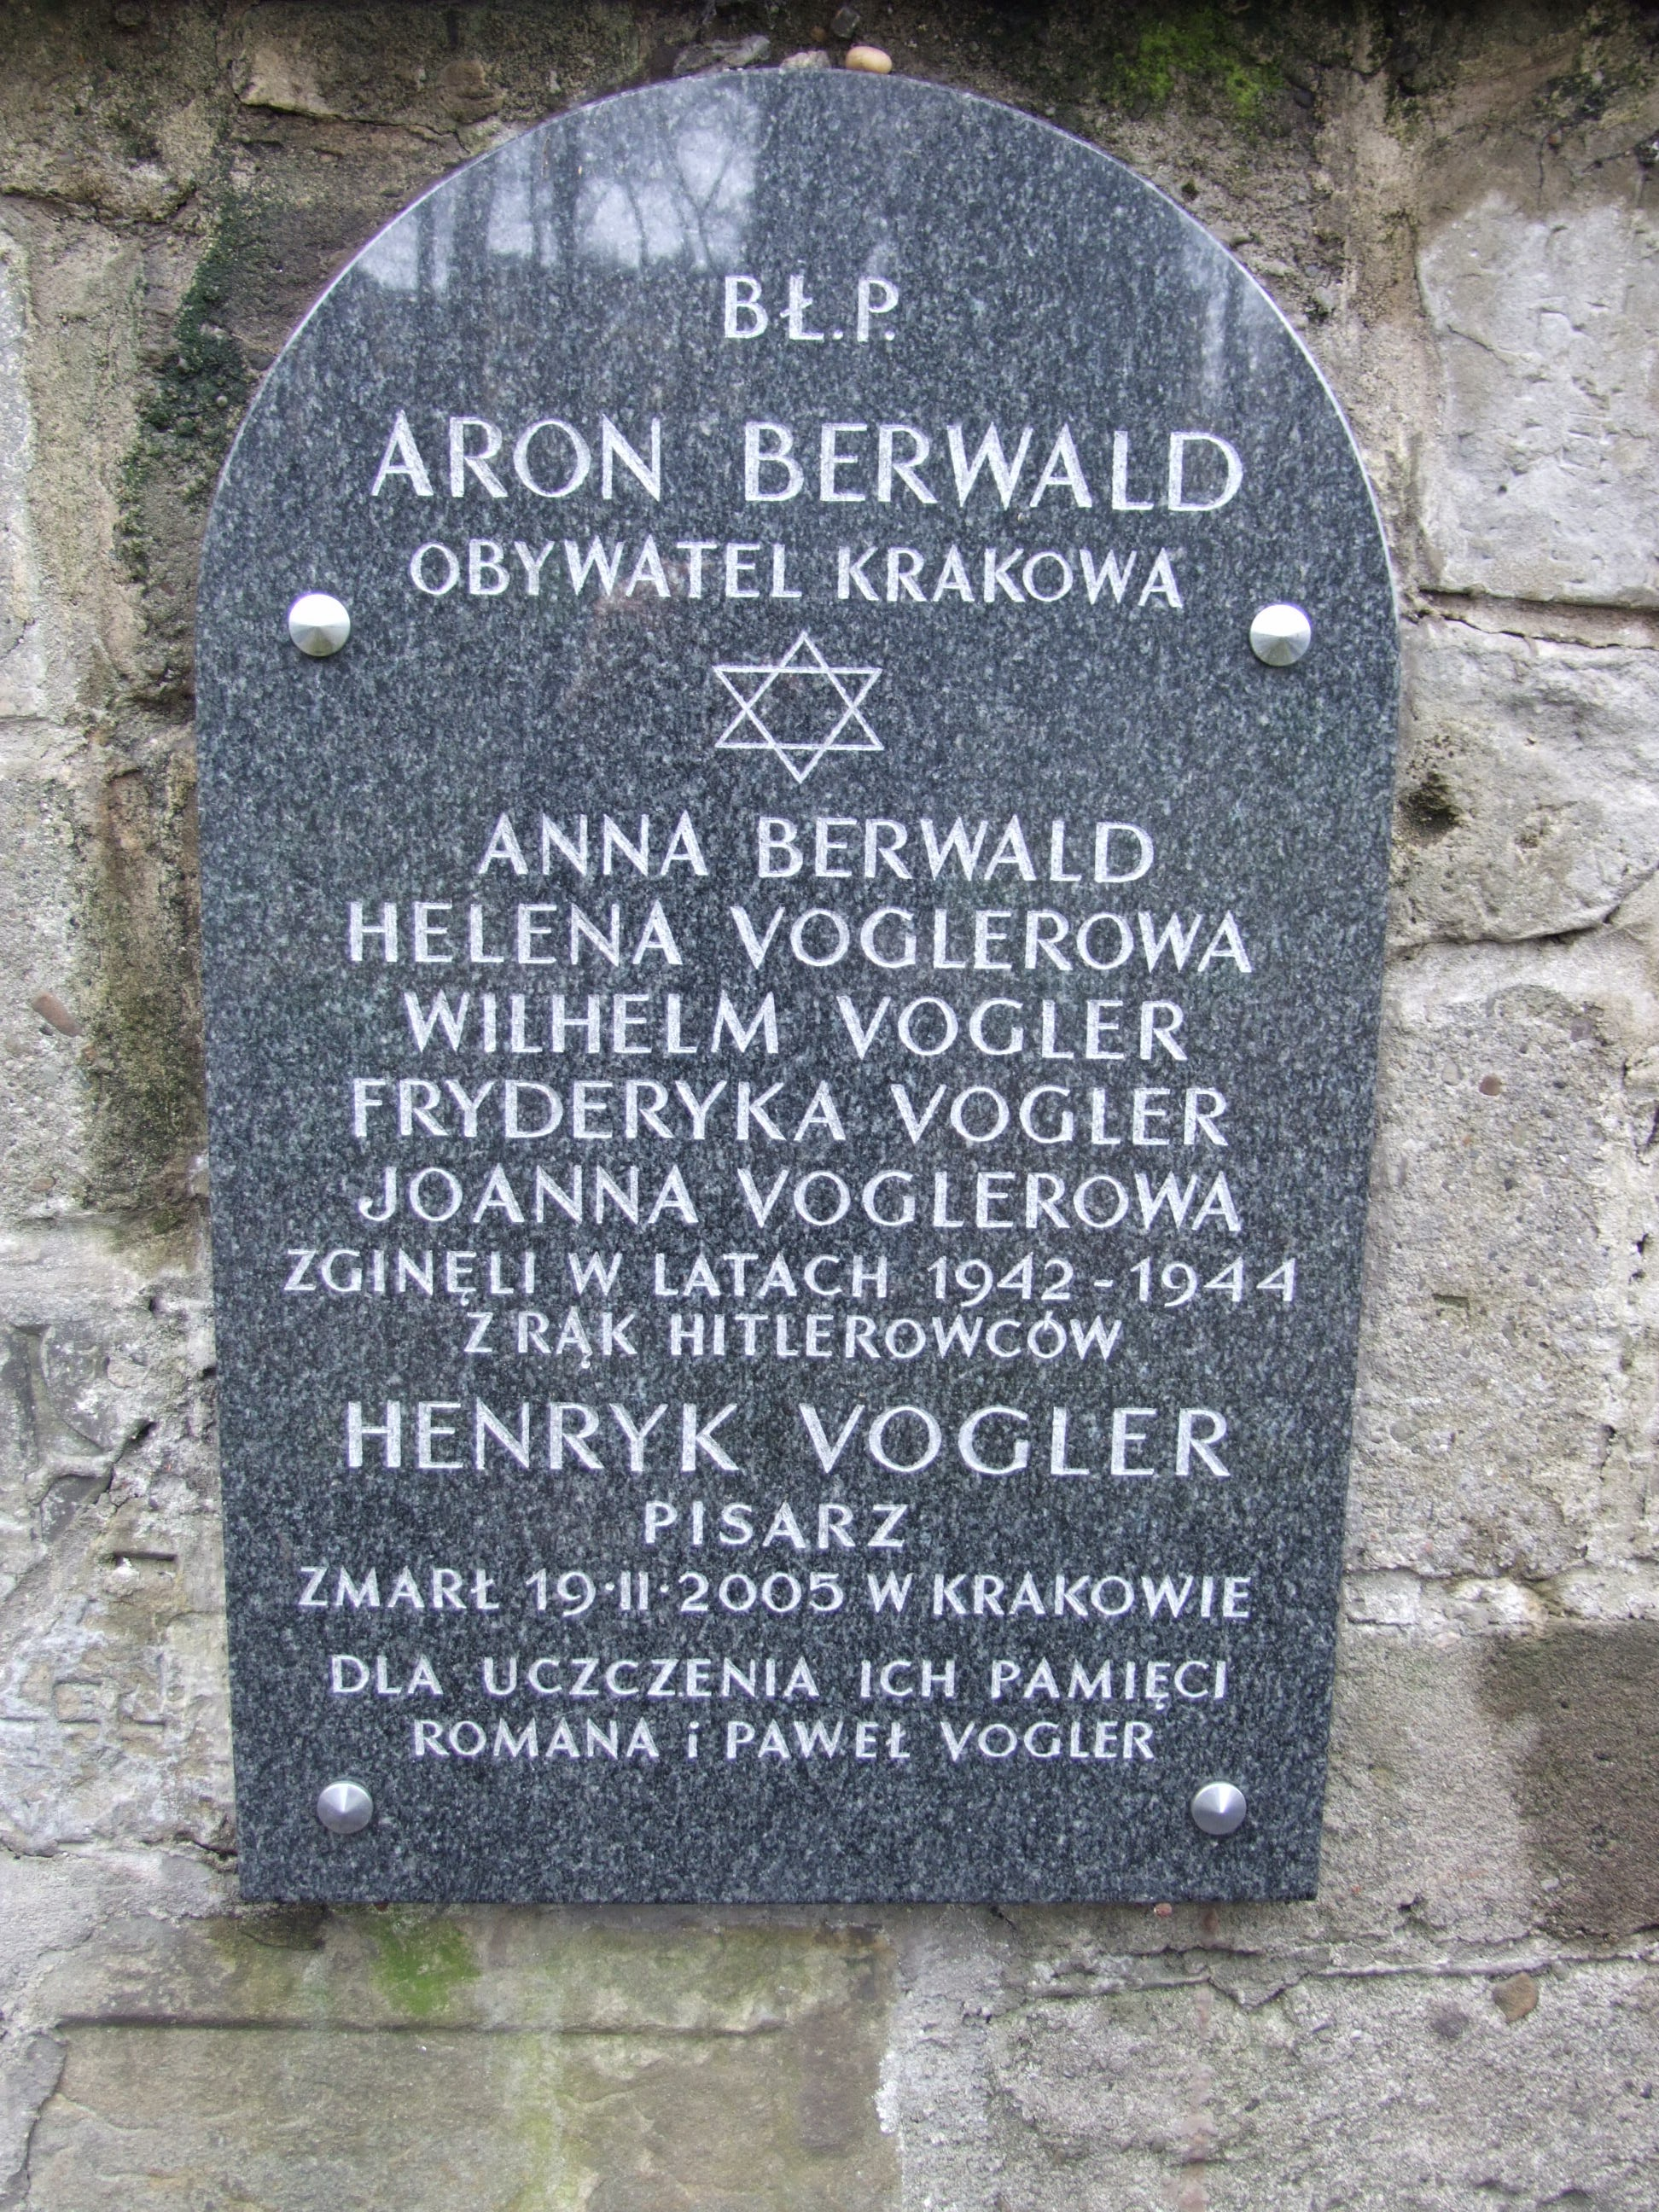
\includegraphics[width=.6\linewidth]{images/nk_vogler}
    \caption{Grab Henrik Vogler auf dem Neuen Jüdischen Friedhof zu Krakau}
    \label{voglergrab}
\end{figure}

\section*{Henryk Vogler}\label{vogler}
Gleich einer Zusammenfassung gibt dieser umfassende Bericht des Polen Henryk Vogler\footnote{PMGR 5758 / 734 / DP. Hier in einer gemeinschaftlichen Übersetzung aus dem Polnischen von Janina und Justina Schott sowie Teresa und Edyta Krawetkowski und dem Autor.} viel dessen wieder, was zuvor bereits Erwähnung fand, und offenbart gleichzeitig eine Vielzahl sonderbarer Details. Vogler war einst Häftling im KZ-Außenlager Görlitz. Den vorliegende Bericht veröffentlichte er in einer gekürzten Form auch in seiner Autobiographie\footnote{Henryk Vogler: Autoportret z Pamińci.}. Vogler verstarb im Jahre 2005. Sein Grab findet man auf dem Neuen Jüdischen Friedhof in Krakau (Bild~\ref{voglergrab}).  




\subsubsection*{Von Groß-Rosen bis Görlitz}
[...]
Die Nächte verbrachten wir in einem großen Saal ohne Betten und anderen Vorrichtungen, sodass wir auf dem blanken Boden nächtigten, einer neben dem anderen. Es schien, als wäre unser Aufenthalt nur vorübergehend. Eines Tages rief man uns morgens auf den Appellplatz zur Übung einer neuen Zeremonie. Es warteten schon jede Menge gestreifte Divisionen, viele andere kamen noch aus anderen Richtungen hinzu. Es stellte sich nach kurzer Zeit heraus, dass der Platz zum Umladen diente. Man stellte Tische für SS-Männer raus. Es begann der Aufruf der Nummern, welche jeder Häftling nach der Ankunft erhalten hatte - das bedeutet nach dem Baden und der Entlausung. Meine Nummer war, wie bei jedem, auf die linke Brustseite der Jacke  genäht. Meine Nummer war über der 14 Tausend (140\dots). Jeder wurde aufgerufen und musste seinen Beruf nennen. Ich blieb weiterhin Schleifer. Nach Beendigung dieser Aktion begannen sie neue Mannschaftstransporte zu bilden. Die Erfahrenen, die schon viele Monate überlebt hatten, sammelten sich zu einer Gruppe, wurden aber getrennt und neu durchmischt.

Ich und Bolek wurden auf diese Weise getrennt, sodass die letzte Verbindung zur Familie abriss.

In meiner Gruppe fanden sich neben alten Kumpels auch neue Gesichter -- auch erfahrene Gefangene. So kamen wir zum nächsten Transport, dessen Waggons wir schon gut kannten. Diesmal dauerte die Reise nicht lange. Wir fuhren ohne zu ahnen, tief ins fremde, feindliche Land zu gelangen. Auf dem letzten Stück stellte sich heraus, dass wir in Görlitz waren. Heute ist es eine Grenzstadt. Die durchfließende Neiße teilt die Stadt in zwei Teile: der eine Teil gehört zur DDR, der zweite Teil, der den Namen \glqq Zgorzelec\grqq~erhalten hat, gehört schon zu Polen.

In den Jahren 1944--1945 wartete dort ein Vernichtungslager auf uns. 
Baracken, wie sie uns aus Groß-Rosen bekannt waren, bildeten hier die Blocks -- die schon fertig, aber noch nicht bewohnt waren. Hier begann und endete der letzte Teil meines Lebens. Das Vernichtungslager in Görlitz gehörte laut Bezeichnung, Namen und Charakter zur Kategorie der klassischen Vernichtungslager. Dies bezeugten die großen Warnungsbuchstaben KL\footnote{KL steht für Konzentrationslager.}, die an einer Tafel aufgestellt waren und darüber informierten, dass dies ein Nebenlager des Lagers in Groß-Rosen war. Dies bestätigten ebenso die aufgestellten Warnhinweise. Der Zaun stand unter Strom, in jeder Ecke befanden sich Gefangenenaufseher mit Maschinengewehren und nachts angeschalteten Reflektoren auf den hohen Wachtürmen. Die Gefangenenaufseher waren überwiegend Deutsche. In den ersten Monaten stand alles unter der Führund der SS. Am Ende sind bei den Männern bedeutsame Veränderungen aufgetreten; die Männer im besten Alter wurden durch ältere ersetzt, die man zwang SS-Unifornen zu tragen. Aber darauf komme ich später noch einmal zurück. Auf jeden Fall herrschte hier eine strengere Ordnung als im Vernichtungslager in Stalowa Wola\footnote{Im Generalgouvernement nahe der Gemeinde Stalowa Wola (Polen) existierte von Juni 1942 bis September 1944 ein Arbeitslager, in dem ausschließlich Juden für eine Filiale der Hermann-Göring-Werke (Stahlwerke Braunschweig) arbeiten mussten.}\index{p}{Stalowa Wola}. Der Appell war gleich dem in Groß-Rosen, zur Arbeit wurden wir von den Wachleuten begleitet, die gleichmäßig und laut im Rhythmus \glqq Links, links, links und links\grqq~schrien.
Die ganze Kolonne wurde zur Arbeit in die Fabrik WUMAG geleitet. WUMAG war die Abkürzung der Firma \glqq Waggon und Maschinenbau Aktiengesellschaft\grqq, also eine Aktiengesellschaft die Waggons und Maschinen produzierte. Aber während des Krieges diente die Firma ausschließlich der Herstellung von Panzergeschossen und Granaten. Die Art meiner Arbeit in der Fabrik war ganz untypisch. Am Anfang lief alles normal. Bei der Registrierung hatten die Deutschen kein Interesse an unserer beruflichen Qualifikation. Es kann sein, dass sie dachten, es sei nicht so problematisch. Freie Plätze wurden von Häftlingen besetzt und von denen gab es genug.

Die Armee Hitlers wurde langsam kleiner, neue Soldaten brauchte man ständig. 
In dieser Zeit stieg ich zum Schweißer um. Unter Anleitung eines älteren deutschen Meisters nahm ich Arbeitskleidung und Maske der richtigen Arbeiter an. In Wirklichkeit war es nur wenig Arbeitskleidung und eine kleine Maske. Mein Gesicht habe ich mit einem Blech verdeckt, um mich vor der Erblindung, den grellen Strahlen und den sprühenden Funken zu schützen. Den Brenner schob ich schon bald durch das Metallstück. Stolz schaute ich mir die violett glänzenden Nahtstellen an, die wie heilende Narben aussahen.

Diesen Beruf übte ich nicht lange aus. Später wurde ich mit weniger verantwortungsvollen Aufgaben betraut; zum Beispiel dem Sortieren von fertiggestellten und silbrig glänzenden, spitzförmigen Geschossen. Als ich manchmal die glatten, vollen Stahlstücke berührte, hatte ich ihre weiteren Wege und Ziele vor Augen; insbesondere, wo sie am Ende landen. Aber ehrlich gesagt, diese Vorstellungen kamen mir selten. 
Man musste diese Aufgaben vor allem ordentlich ausführen. Diese Arbeit dauerte nur bis Ende 1944. Gerade in dieser Zeit begann der untypische Wandel. Ich wurde in einem Fabrikbüro als Kanzleiarbeiter eingestellt. Der Gefangenenstatus hatte sich für mich verbessert, obwohl ich die Hälfte der 24 Stunden in der Fabrik verbringen musste. Die Bedingungen der zweite Hälfte der 24 Stunden waren wie bisher, obwohl ich zugeben muss, dass es nach der Ernennung gut für mich aussah -- man achtete und schätzte mich.

Im Büro vertraute man mir die Anlegung und Führung von Akten der in der WUMAG beschäftigten Häftlinge an, also ihre persönlichen Daten und Registrierungen der Arbeitsplätze, welche sie auf den einzelnen Strecken besaßen. Das war eine normale Registrierung, aber es hatte keine Bedeutung und auch keine Vor- und Nachteile für die Gefangenen, es spielte eben keine Rolle.
Tatsächlich mag so ein Register komisch aussehen, ebenso mag der Anblick eines mageren Arbeiters in weiß-blauem Sträflingsanzug und Holzschuhen mit Glatze und einem Haarstreifen mitten auf dem Kopf von Stirn bis Nacken für den, der am Bürotisch oder an der Schreibmaschine saß, komisch ausgesehen haben. Diese Haarschnitte wurden ihnen sofort beim Eintritt ins Lager gemacht; vielleicht weil jeder Fluchtversuch schon von vornherein zum Scheitern verurteilt werden sollte.
Es ist für mich schwer nachvollziehbar, weshalb es für mich solch eine glückliche Wendung nahm. Es ist nicht ausgeschlossen, dass der eben erwähnte alte Meister etwas damit zu tun hatte.

Am Anfang machte er den gefangenen Fabrikarbeitern Angst. Er lief von einem zum andern und wirbelte gefährlich mit den Händen über Ihnen herum. Sein grauer Kopf wackelte schon vor Aufregung, er schrie sehr laut und beschimpfte diejenigen, die ihm ein Dorn im Auge waren. Manchmal konnte man wegen seines Dialekts kein Wort verstehen. Doch schon bald wurde klar, dass es nur so schien. 
In Wirklichkeit erwies sich der Meister als warmherzig, er machte sich Sorgen um das Schicksal seiner Arbeiter, die er in Wirklichkeit nie verletzt und angegriffen hatte. Manchmal hatte er den Arbeitern heimlich Essenspakete zugesteckt ohne zuzugeben, dass er es war. Manchmal murmelte er etwas zu mir, obwohl ich kein Wort verstanden habe. Man konnte nur vermuten, dass er früher ein Mitglied der sozialistischen Partei gewesen und Hitlers Gegner geblieben war. Bei Gelegenheit erfuhr er von mir  meinen richtigen Beruf und meine Qualifikationen. Sicherlich erfuhr die Fabrikleitung von meinen Qualifikationen durch ihn und so kam es zu dieser unerwarteten Anstellung.

Mein Vorsitzender im Büro hieß Tschornak - sein Name wurde wahrscheinlich in vorherigen Generationen Czornak geschrieben oder einfach nur Czerniak. 
Das bewies seine slawische Herkunft, um genau zu sein, seine sorbische Herkunft. Er hat es nicht verneint. Solche ähnlichen Fälle gab es häufig in der Fabrik, so dass man sich an Arbeiter wie Szepaniak, Zebulla oder Roch erinnert. Tschornak, ein stattlicher Mann für sein Alter, war ein Kriegsversehrter des ersten Weltkrieges; er hatte keinen linken Arm, der aber durch eine Prothese ersetzt und mit schwarzem Leder überzogen war.
Er gehörte zur Partei, da er an seiner Jacke ein kleines, rundes Zeichen mit Hakenkreuz trug, doch er war freundlich zu mir, ja man kann sagen fürsorglich. 
Er verhielt sich höflich, wie zu einem geliebten Schoßhündchen und nannte mich immer \glqq Heinrich\grqq.

Manchmal unterhielt er sich mit mir über ernste Themen: neugierig fragte er mich  über meine Vergangenheit aus. Er versuchte heikle Themen zu umgehen, etwa die Gründe warum ich hier bin. Überhaupt hatte das Verhältnis zum Meister und zu einigen deutschen Arbeitern  für uns einen besonderen Charakter. Es gab auch solche wie Brochmann oder Bochmann, seinen Namen merkte ich mir nicht genau, die uns brutal behandelten, wenn sie mit uns unzufrieden waren. Sie schlugen uns und waren sichtlich befriedigt.

Aber die Mehrheit verhielt sich gegenüber den jüdischen Arbeitern ein bisschen so, als wenn sie nicht existieren. Sie wichen ihren Blicken aus, sie schauten nach oben und zur Seite, es ließ sie kalt. Außerdem unterließen sie Kontakte während der Arbeitszeit -- unsere Existenz und ihrer Probleme interessierten sie nicht. 
Man hätte denken können, dass sie von der Existenz des Lagers, aus dem sie täglich extra Arbeitergruppen unter Aufsicht eskortierten, nichts wussten. Das Lager existierte auf jeden Fall und zwar mit einer ganz perfekten Organisation, wie ich sie bis zu diesem Zeitpunkt noch nicht erlebt hatte. Einmal erinnerte ich mich daran, dass Hitlers Lager eine Art separater Staat mit eigener Gemeinschaft und klassischer politischer Struktur war. Am deutlichsten empfand ich dies in Görlitz.

Natürlich gehörte die ganze Macht der SS. An der Spitze der Macht stand der Lagerführer Zunker. Er erinnerte mich an einen Sturmmann aus Rozwadow\index{o}{Rozwadow}\footnote{Seit 1973 ein Ortsteil von Stalowa Wola, Polen.}, doch er war merklich größer, mit Charge und Reife. Das Todesurteil, das er aussprach und vollstreckte, war frei von momentanen Emotionen oder Wahnsinn, dafür aber kaltblütig durchdacht. Gleichermaßen waren die deutschen Soldaten Angehörige der SS, welche die Wachmannschaften stellten, jedoch besaßen sie nicht solch grausame Phantasien der Rozwadower\index{o}{Rozwadow} Ukrainer, dafür aber Ordnung und Konsequenz, die noch schlimmere Konsequenzen mit sich brachten. Am Anfang schienen sie fast wie Halbgötter mit Totenkopf auf dem Kragen. Doch wenn es zu einer zufälligen Annäherung kam, erschienen sie wie unberechenbare Bestandteile des Erdreichs. % (nicht vorhersehbare Erdelemente)

Für mich war zum Beispiel bereits ein kleiner Vorfall bedeutsam: In einer bestimmten Zeit vor Beginn meiner Arbeit im Büro gehörte ich zur Gruppe, die täglich zu Mittag einen Kessel mit Suppe für Kameraden austrug. Diese Aufgabe wurde immer anderen Häftlingen zugetragen, um zu verhindern, dass jemand bevorzugt wird. Diese Beschäftigung, um die sich jeder eifrig bemühte, war sehr begehrt: Sie berechtigte zu einer Prämie in Form einer zusätzlichen Suppenkelle. Dieser Kesseltransport fand unter der Aufsicht von SS-Soldaten statt, welche uns eskortierten. Für mich waren sie ohne Gesicht -- meine Angst erlaubte es mir nicht auf sie zu schauen, sie hätten es bemerken könnten und es hätte schlimme Folgen gehabt. Alle blieben in der unpersönlichen, übermenschlichen Gestalt.
Eines Tages wurde eine Gestalt  wieder lebendig, das Gesicht hatte sinnliche Form angenommen. Nach Beendigung der Mahlzeit brachte ich den letzten leeren Kessel in den dafür vorgesehenen Raum zurück. Ein paar Sekunden später kam mir ein SS-Soldat mit Maschinengewehr hinterher. Wir waren nur zu zweit. Ich schaute auf den bewaffneten Soldaten und hielt meinen Atem an, er lief in meine Richtung. Er kam mir immer näher, seine Augen waren groß und aufgerissen. In diesem Moment wurde er zum Mensch, ich sah wie klein und häßlich er war, mit kaputten Zähnen und erdiger Haut. Plötzlich presste er seinen Körper an mich, oder vielmehr seine Uniform, zitternd und schnaufend flüsterte er mir ins Ohr: \glqq Du bekommst Suppe\grqq.

Mit flatterndem Herzen auf das Gewehr schauend, gelang es mir zu fliehen. 
Ich lief von dieser überraschenden Lagerliebe davon, murmelnd sagte er, ich soll sofort zur Arbeit zurückkehren.

Ich weiß nicht, ob diese Geschichte den Wechsel oder das normale Bild innerhalb der SS-La\-ger\-mann\-schaften, sozusagen den Zustand des Verbandes widerspiegelt.

Auf jeden Fall wurden die Veränderungen langsam offensichtlich. Die bisherigen Wächter wurden an die Front geschickt um die Lücken der deutschen Armee zu füllen. An deren Stelle kamen ältere Bewohner aus der Umgebung; man zog ihnen SS-Uniformen an und machte aus ihnen Soldaten und Lagerwächter. So war das auf jeden Fall in Görlitz.

Man muss sagen, dass die neuen SS-Männer einst ruhige Einsiedler und Kaufmänner oder Handwerker waren, sie versuchten ihre Pflichten so gut es ging zu erledigen. Es war komisch, dass die Mehrheit von ihnen keine Ahnung hatte, dass der Krieg bald zu Ende ist.

Ich erinnerte mich zum Beispiel an einen warmherzigen Rapportführer, der grau wie eine Taube war.  Sein großer Bauch war mit einem Ledergürtel umgeben, an dem sich ein Etui mit Pistole befand. Der ältere Mann kam mir sympathisch entgegen. Es kann sein, dass er auch zu anderen Häftlingen nett gewesen ist, aber darüber weiß ich nichts zu sagen. Er versuchte mich vor schweren Lagerarbeiten zu bewahren und manchmal steckte er mir eine zusätzliche Brotscheibe oder andere Lebensmittel zu; ich betone nur manchmal, damit ich die Lagerarbeiten überstehe.

Manchmal saßen wir nach dem Abendappell zusammen und unterhielten uns. 
Das war wahrscheinlich schon im März 1945, die ersten Frühlingszeichen zeigten sich. Der Rapportführer ahnte die Niederlage der Deutschen und hielt Hitler für schuldig, dass das Land zerstört wurde. Bei früheren Gesprächen fragte ich ihn, was er machen würde, wenn er den Befehl bekommen würde mich zu erschießen.
Der alte Mann schwieg und ich sah vor mir seine klaren, blauen Pupillen, die sich vor Erstaunen immer mehr ausweiteten. Dann sagte er freundlich und treuherzig bei klarem Bewusstsein: \glqq Wie ich es machen würde? Natürlich würde ich dich erschießen. Befehl ist Befehl.\grqq

In dieser Zeit ereigneten sich sporadisch Erschießungen auf dem Lagerplatz und man versuchte im Sinne einer Rechtssprechung dem Ganzen einen Rahmen zugeben. Einmal ertappten sie einen Häftling beim Kartoffelklau in der Lagerküche. Man stellte ein Gericht mit dem Lagerführer auf, sie verhörten Köche, danach wurde der Schuldige erschossen. Aber ähnliche Urteile oder Exekutionen hielten die Häftlinge nicht davon ab, sich in die Küche zu schleichen und nach Essen zu suchen. Die Hungerseuche verging nicht, zumal der Nahrungsbedarf größer und vielseitiger wurde. Ab und zu gab es sogar Wurststücke. Innerhalb kurzer Zeit bekamen wir Zigarettenrationen, welche gefragt waren, um sie gegen Lebensmittel einzutauschen.

Aber nach Jahren eines schwächer werdenden Immunsystems war das Nervenzentrum durch den Hunger physiologisch zunehmend gelähmt und immer weniger zu anderen Regungen fähig, als jenen, die das Essen bezweckten.
 
Beispiele gibt es genug, aber eines erscheint mir außergewöhnlich. Vorher wäre es vielleicht notwendig, kurz die Charakteristik des Ordnungsgefüges der Lagergesellschaft zu erklären. Es herrschte eine Hierarchie, welche dem Lager eine Art Autonomie verschaffte. Große Macht besaßen die Blockältesten, denen einzelne Blöcke gehörten und von denen es genug gab. Auf der niedrigsten Stufe der Leiter stand der Verantwortliche für die einzelne Baracke (Stubendienst, dazu gehörte zum Beispiel die wichtigste Tätigkeit: das Suppeaustragen). An der Spitze stand der Lagerälteste. Diese Stelle besaßen Häftlinge, die einfache Kriminalverbrechen begangen hatten -- dies bewies ein rotes Dreieck am Sträflingsanzug. Mit dieser Rechtfertigung haben ihnen die Überlegenen aus politischem Kalkül vieles mit Brutalität zu verstehen gegeben.

Unser Lagerältester hieß Czech. Seinem Vornamen nach war er ein Deutscher -- ein alter schlauer Fuchs, der sich seit Jahren schon im Lager befand -- wahrscheinlich wegen Mordes. Er war klein und machte den Eindruck eines Zwerges mit einem großen Kopf, seine Lippen waren bissartig verbogen und sein leicht schielender Blick schaute über die Brille hinweg. Seine Augen verrieten zweifellos eine Intelligenz, die sich bei der Misshandlung von Häftlingen erfinderisch zeigte. Zur Hilfe hatte er zwei Lagerkapos, welche große Macht hatten. Die beiden stammten aus dem Lager Stalowa Wola\index{o}{Stalowa Wola}. Einer hieß Tennenbaum -- ein primitiver Halbanalphabet -- er arbeitete im Stahlwerk, niemand achtete dort auf ihn und erst im Konzentrationslager Görlitz entdeckte man seine Begabung und Eignung, die ihn in den Lagerrang erhob. Der zweite, an den man sich auch erinnerte, hieß Schneebaum -- ebenso wie die Funktion eines Arztes hatte er die des zweiten Lagerkapos inne, und wenngleich Tennenbaum viel Brutalität an den Tag legte, vollführte er sie auf eine intelligente Weise. In Klammern gesagt, die erstaunliche Persönlichkeit von Schneebaum erlaubte es mir damals Phänomene zu entdecken, die als unbegrenzte Möglichkeiten in einem Menschen vorborgen sind. Welch seltsame Begebenheit, dass ihre Namen die gleiche Endung \glqq Baum\grqq~besaßen.

Sie brachten mich auf die Idee einer Satire. In letzter Zeit versuchte ich mich zu bemühen eine Art Theaterstück zu schreiben und schließlich eine Lagerbühne zu montieren. Ich spielte vor Kameraden aktuelle Stücke und Monologe in deutscher Sprache, da unsere Gesellschaft multinational war und weil es die einzige Möglichkeit war sich zu verständigen.

Ein berühmtes deutsches Weihnachtslied: \glqq O Tannenbaum! \dots\grqq~sang ich abwechselnd: \glqq Tennenbaum\grqq~statt \glqq Tannenbaum\grqq~-- spöttisch lachte man über den Lagerkapo.

Die Ähnlichkeit der Namen benutzte ich für ein Wortspiel: Wenn der Winter anbricht, Schnee die Bäume bedeckt und dann den Tannenbaum, so wird aus Tennenbaum ein Schneebaum. Dieser Text erreichte den Lagerältesten, welcher mich zu sich rief und mich verhörte. Aus seinen verdächtigen und hinterlistigen Fragen schloss ich, dass meine unschuldige, satirische Idee das Geheimnis innerer Kämpfe um die Macht im Lager verriet, und Czech nun befürchtete, dass ich eine Rolle im politischen System (von dem ich in Wirklichkeit keine Ahnung hatte) spielen wolle. Die Nichtahnung beschützte mich vor Auswirkungen, die es für mich hätte  haben können.

Aber jetzt ist es an der Zeit zum eben angekündigten Vorfall zurückzukommen, bei dem ich auf die besondere, magnetische Kraft des Hungers eingehe. Eines Tages wurde einer der Häftlinge zu 25 Schlägen verurteilt; wofür weiß ich nicht. Der Lagerälteste führte es aus. Obwohl er wie jeder andere auch ein Häftling war konnte er seine Funktion zur Erlangung entsprechender Vorteile und Vorrechte ausüben -- genau wie dies alle anderen in der gleichen Position als natürlich empfanden. Er hatte ein extra Zimmer, das komplett mit einer Vorratskammer eingerichtet war.

Der Verurteilte musste sich ausziehen und sich auf die extra vorbereitete Bank legen. Sein Kopf hing an einem Hängeregal herunter, auf dem ein halbes Brot lag. Als der Lagerälteste zu schlagen anfing, spürte der Häftling keinen Schmerz, weil er vor sich den herrlichen Anblick und Duft des Brotes vernahm, der seinen Schmerz neutralisierte. Während seiner schweren Schläge biss er gleichzeitig mit seinen Zähnen saftige Stücke ab, schnell schluckte er Stück für Stück und betete, dass die Exekution so lange wie möglich weitergeht. Mit voller Begeisterung und ohne etwas auszulassen erzählte er uns alles; auch vom Leid, dass so schnell vorüber ging.

Man muss zugeben, dass Czech in diesem Fall Sinn für Humor bewies. Als der Lagerälteste mitbekam, dass etwas Brot fehlte, wusste er gleich was los ist. 
Nach kurzem Überlegen lachte er wie über einen Scherz. Wenn sie Hunger hatten, versuchten sie alles mögliche um den Hunger zu befriedigen. Einmal brachte eine Gruppe meiner Kumpels aus meinem Block auf dem Weg von der Arbeit einen Hund mit. Sie entführten ihn auf der Straße und führten ihn durchs Tor; das hätte schlimme Folgen haben können. In unserem Block hatte ein kleiner, grausamer, strenger Metzgergeselle namens Matias, über den ich später noch erzählen werde, die Macht. Durch die Mithilfe einiger Kumpels hatte er es schnell und gut organisiert, den Hund zu erschießen. Er zerstückelte ihn mit geeigneten Werkzeugen und mit der Hilfe der Köche bereiteten sie ihn zu. Ein ausgewählter Kreis verzehrte die gemeinsam zubereitete Speise. Dank eines Anwesenden gelang es mir auch davon zu kosten. Ich bekam ein Knochen, der mit Fleisch bedeckt war. Es schmeckte mir so sehr, wie nichts anderes danach. Die Sache war ein Geheimnis und konnte für die Teilnehmer des Festmahls nicht ohne Folgen bleiben. Es wäre gar nicht erst so weit gekommen, wenn der Lagerälteste nicht mit daran Teil genommen hätte. Er bekam einen Teil der Beute: Hundefett, von dem Kenner behaupteten, es besäße wichtige Nähr- und Heilwerte. Es war nichts Außergewöhnliches, dass der Lagerälteste bei allem ein Auge zudrückte, obwohl es hätte Konsequenzen haben können.

Ich habe einige Fälle geschildert, was man alles versuchte, um an zusätzliche Nahrung zu gelangen. Aber die unheilbare, chronische Hungerzeit dauerte schon drei Jahre an. Zum Hunger kam in der letzten Zeit eine neues, unbekanntes Produkt hinzu. Später transportierte man kein Salz mehr nach Görlitz ins Lager. Suppen und andere Nahrungszuteilungen mussten ohne dieses Gewürz auskommen. An dessen Stelle teilte man große kupfer-gelbe Blöcke aus; sie erinnerten an Felsstücke, die man zerkleinern musste, um ein Pulver zu bekommen, dass man dann als Gewürz benutzte. Man nannte das Gewürz Tiersalz. Dieses Gewürz erhielt einen minimalen Prozentsatz Küchensalz. Ich habe erkannt, was ich vorher nicht wusste, dass Salz ein wichtiger Nährstoff für den Organismus war. Die letzten Monate in Görlitz waren eine Qual ohne dieses Gewürz und alles, was man herunterschluckte, verlor an Wert. Die ganze Zeit habe ich dieses quälende, schmerzvolle Gefühl erfahren müssen, gleich einem Drogensüchtigen ohne seinen Stoff. Ich hätte mein Leben aufgegeben, nur um noch einmal an einem salzigen  Kristall zu lecken. Zu diesem Zeitpunkt wurde der Hunger vielfach größer. Fakt ist jedoch, dass mein Körper seit dieser Zeit und bis heute ein gefräßiges Verlangen nach Salz hat. Man lacht mich aus, weil ich bis heute Unmengen an Salz nutze. Dieser Tatbestand führte zum Tode mehrerer Häftlinge im Lager. 


Ende 1944 und Beginn 1945 war es soweit, dass man mit dem Beerdigen nicht hinterher kam. Deshalb hatte man die Leichen in die Vorratskammer gebracht und gestapelt, damit man sie wenigstens einmal die Woche auf einen Schlag wegschaffen konnte. Einmal war ich auch beim Entsorgen dabei. Vor die Vorratskammer stellte man einen Holzwagen, auf den man die nackten Leichen auflud. An diesem Tag gab es dutzende Leichen. Ein Teil unserer Gruppe zog den Wagen an der Deichsel, der andere Teil schob. So schoben wir den Wagen durch die Stadt auf den Friedhof\footnote{Jüdischer Friedhof zu Görlitz.}, wo ein großes ausgehobenes Grab wartete. Wir schoben die Leichen vom Wagen - einen auf den anderen. Sie waren schon Haut und Knochen. Als sie aufeinander fielen, klang es, als wenn man es mit Skeletten zu tun gehabt hätte. Die vergangenen kalten und kühlen Tage hatten die Leichen, die ohnehin schon ganz ausgetrocknet waren, konserviert. Ich schaute in die offenen Augen meiner Kumpels, mit denen ich noch vor ein paar Tagen zusammen von der Arbeit kam. Sie verwandelten sich in steife Körper, die man wie Puppen nach unten schmiss. Nach dem Zuschütten des Grabes mussten wir nebenan ein neues Grab ausheben. Ich erfuhr, dass es immer so gemacht wurde, um Zeit zu sparen. Dank dieses Systems waren die Gräber für die nächsten Ladungen vorbereitet.

Am Ende unserer Arbeit kam es zu einer überraschenden Begegnung. Der Friedhof war klein und ruhig; wahrscheinlich hatte man ihn schon lange Zeit nicht mehr genutzt und wenn, dann sicher nur für Lagerhäftlinge aus der Umgebung. Der Ort hatte etwas von einem Museum und von einem Denkmal. Im Abstand aufgestellte Steindenkmäler schienen wie gemeißelte Kunstwerke, deren unscharf verschwommene Gotikschrift im Laufe der Zeit mit Patina überzogen war. Hier wehte wirklich der Tod - vielleicht weil die Wege mühsam mit Kies bestreut, das Gras gleichmäßig gemäht und mit Blumen geschmückt war. Man spürte überall, dass sich jemand darum kümmerte. Dieses Gefühl machte sich bemerkbar, als sich ein älterer, magerer Mann geheimnisvoll an uns heran schlich. Erst nach einem kurzen Gespräch stellte sich heraus, dass wir uns auf einem fast hundertjährigen jüdischem Friedhof befanden, um den sich die Behörden nicht mehr kümmerten. Aber ein deutscher Gärtner\footnote{Gemeint ist Otto Pfeffer.}\index{p}{Pfeffer, Otto}, der jeden Tag aus eigenem Interesse hierher kam, kümmerte sich stellvertretend für Familienangehörige, die es nicht mehr gab, um die Gräber und hielt Ordnung. Dank ihm glich das Bild des Friedhofs einem gepflegten Park, obwohl er verlassen war. In jenem Moment beugte er sich, klein und zierlich wie ein Vogel, zu uns und flüsterte uns lachend zu:  \glqq Ich wache hier. Wenn die Familien wieder zurückkehren, finden sie es vor wie sie es verlassen haben.\grqq

Ich erinnerte mich, dass jede Woche massenhaft Beerdigungen stattfanden. Obwohl sie verstarben, merkte man es nicht, da immer wieder Transporte mit neuen Gefangenen hinzukamen. Sie kamen zu verschiedenen Zeiten und aus verschiedenen Richtungen. Ein Transport war von außergewöhnlicher Art und für den weiteren Verlauf in Görlitz bedeutsam. Ich spreche über einen Frauentransport aus Ungarn, der im Spätherbst, Oktober oder November 1944, zu uns kam. Sie wurden im Lager getrennt vom Männerlager untergebracht,  sodass uns der Drahtzaun einige Meter voneinander trennte. Erschien man in der Nähe der Frauen -- überwiegend jüngere, arbeitsfähige Mädchen -- löste es eine Erschütterung aus.

Ab diesem Moment ergaben sich zwei Arten von Geschlechterproblemen im Lager.
Es war als wenn die lang andauernde Isolation der Frauen einen Liebeshunger verursachte, der ebenso intensiv wie der Hunger aufgrund fehlender Lebensmittel zu sein schien. Zu dieser Zeit stellte ich fest, dass es bei mir umgekehrt war. Das Verlangen erlosch Jahr für Jahr mehr.

Übrigens fällt mir auf, ich habe es nicht genau durchdacht und nicht richtig überlegt, welche Art von Problemen es hätte haben können. Ich war wie jeder andere auch damit beschäftigt, wie ich eine zusätzlich Portion Suppe oder eine Kartoffel bekomme konnte. Es stellte sich heraus, dass der erste Hunger [nach Nahrung] wichtiger war, als der andere \glqq Hunger\grqq~[nach Liebe], welchen der Gelehrte Freud\footnote{Sigmund Freud.} mit den anderen gleich stellte. Seit ich mich in Görlitz befand, war ich ein geschlechtloses Wesen. Es stellte sich heraus, dass einigen -- vor allem Funktionshäftlingen, die nicht vom Hunger betroffen waren -- entsprechend dem hier Aufgeschriebenen, die Bereitschaft zur Sexualität nicht verloren gegangen war. Dies hatte natürlich Folgen. Der von mir eben schon erwähnte Kapo Matias zum Beispiel hatte einen schlanken, blassen Jungen mit Augenringen zur Verfügung, der nicht nur tagsüber seiner Pflicht nachging, sondern sich auch im Tausch gegen Vorrechte zusammen mit Matias die Pritsche teilte.

Jetzt aber überkam mich beim Anblick der Mädchen eine bislang unbekannte Erregung. Es war nichts Sinnliches dabei, der Körper war taub und reagierte nicht. An meine Jugendzeit erinnert, rührte es mich innerlich, als ich die herannahenden Mädchen sah; das Herz und die Kehle drückte mir und ich wusste nicht aus welchem Grund. Jetzt mag es einem merkwürdig erscheinen, dass wir die Weibsbilder in Sträflingsanzügen heimlich durch Stacheldraht beobachteten, wie sie regelmäßig ihre Märsche absolvierten -- unter Aufsicht einer deutschen Lagerführerin mit einer männlichen Gestalt, die nichts Besonderes, Attraktives an sich hatte.

Der Eindruck war stärker, wenn man sie aus der Nähe sah. Ein Teil von ihnen war in der WUMAG beschäftigt. Ich konnte mehrmals am Tag an ihnen vorbeigehen, weil sie an Maschinen und im Lager arbeiteten, aber es war uns verboten mit ihnen zu sprechen. Es schien als hätten sie keine Merkmale einer Frau; sie hatten keine angepassten Sträflingsanzüge und laut Vorschrift mussten ihre Köpfe kahl rasiert sein. Jedes Mal, wenn ich mich kurze Zeit in ihrer Nähe befand, floss zwischen ihnen so eine Art Strom. Nach kurzer Zeit wuchsen ihnen die Haare wieder nach und sie wurden nicht mehr rasiert. Einige von ihnen waren mutig und setzten sich ein Kopftuch auf, um auf sich aufmerksam zumachen. Auch in den Sträflingsanzügen konnte man Anzeichen schüchterner Koketterie bemerken. Langsam entdeckte man die Funktionen der Augen und Lippen sowie die Merkmale der weiblichen Anatomie.

Als Büroarbeiter hatte ich Gelegenheit mich jederzeit in der Halle zu bewegen und in jeden Winkel zu schauen, um Informationen zu sammeln, da ich über jeden Kartei führen musste. Manchmal, wenn die deutschen Meister nicht in der Nähe waren, gelang es mir ein paar schnelle Worte mit den exotischen Wesen zu wechseln. Unter ihnen befand sich eine Ungarin mit funkelnden schwarzen Augen, dunklerer Haut und kleinen Lippen mit einem kindlichen Lächeln. Sie hieß, wie ich erfahren habe, Hojnolka - der Klang ihres Namens erschien mir seltsam schön wie sie selbst. Sie arbeitete an einer Maschine; später ergab sich zwischen uns eine Romanze. Diese Romanze bestand aus dem Austausch unserer Blicke und kleiner Zettelchen, auf denen unsere Gefühle auf deutsch geschrieben standen.
Hojnolka schrieb weniger, das meiste kam von mir und bot mir Gelegenheit mich literarisch auszuleben. Die Rolle eines Liebesbriefträgers übernahm eine mitgefangene Ungarin, die die Hallen reinigte. Sie war hässlich, mit einem breiten Gesicht und einer schiefen Nase. Dies ermöglichte mir den Kontakt zu ihr, trotzdem der ausgesetzten Gefahren. Einmal wurde sie fast von Bochmann bei einer Tat erwischt, doch dank ihrer Schnelligkeit blieben [ihr] die Konsequenzen erspart.
Ich war nicht der einzige, den der neue Zauber und das Interesse der Frauen anzog. Manche Häftlinge suchten sich von weitem und durch den Stacheldraht ihre Frauen aus, die sie dann mit Sehnsucht anschauten. Erstaunlich, wie viele schmutzige, verlauste Männer es gab, die nur zur Brutalität neigten, seit Jahren gehorsam ihrem Instinkt folgten und doch noch ein empfindsames, sentimentales Innenleben hatten. Vielleicht bildeten dies einen wichtigen Bestandteil einer psycho-physischen Kombination namens Mensch, aber vielleicht ist es ein unterschwellige hervorgerufene Sexualität. In diesem Geisteszustand waren manche bereit, sich dem Großen zu widmen. Unter Anwendung der vorhandenen Möglichkeiten und Tricks hielt sie nichts davon ab, Lebensmittelpäckchen für ihre auserwählten Frauen zu schmuggeln; oftmals haben sie auf Essen verzichtet, um ihre Gefühlsstärke zu beweisen.
Meine Romanze in schriftlicher Form mit Hojnolka dauerte eine Weile bis es unerwartet zu einem echten Kontakt kam. Es geschah in Verbindung allgemeiner Vorfälle. 

Am Anfang als der Krieg ausbrach, glaubten wir alle weit von ihm entfernt zu sein. Sein Klang drang nicht bis zu uns vor. Aber Ende des Jahres kam es offensichtlich zu einer Veränderungen. Ich erinnere mich an den ersten Fliegeralarm, der während der Arbeit in der Fabrik ausgelöst wurde. Die Sirenen heulten und unter den Deutschen brach Panik aus. Die Gefangenen bildeten Reihen und panisch drängte man sich in Bunker. Als wir dahin liefen, schaute ich zum Himmel. Weit und sehr hoch über uns flog eine silberne Staffel. Ich begrüßte sie stillschweigend und freudig mit glücklichem Herzen, wartend auf die Offenbarung einer gesegneten Bombardierung. Diesmal traf es nicht zu und der Alarm wurde abgesagt. Ab diesem Zeitpunkt erschienen diese Vernichtungsboten öfters am Himmel und auf Land -- bis zu dem Tag, welcher als der letzte ausgerufen wurde.
Es erinnerte an die Evakuierung von Stalowa Wola\index{o}{Stalowa Wola}, aber es verlief anders. Der Befehl lautete, beide (Männer- und Frauen-) Lager sofort zu verlassen.

Dies geschah in einer großen Eile, die viel Unerwartetes geschehen ließ. In jenem Lärm gelang es mir, mit anderen Häftlingen in die unbewachte Vorratskammer einzudringen und uns die Taschen mit Lebensmitteln zu füllen. Dieser Vorrat sollte uns in Zukunft hilfreich sein. Aber man hörte schon aus allen Ecken deutsches Gerede. Zuerst verließen lange Frauenreihen, und hinter ihnen Männerreihen, die Lagertore.

Es begann ein Ereignis von kurzer Dauer, das zu den dramatischsten in meinem Lagerleben zählt. Auf den Landstraßen und auf den wenig benutzten Wegen schleppten wir uns unter Aufsicht der SS-Männer Richtung Westen. Der Winter war diesmal nicht streng, aber in den dünnen Sträflingsanzügen froren und zitterten wir, da es Schneeregen gab und wir mit Holzschuhen durch den kalten Matsch liefen. Ich ging eingekuschelt in einer kaputten Pferdedecke, die von einer Pritsche herunter genommen wurde. Jeder Gefangene versuchte sich etwas zu besorgen, in diesem Moment wurden die Vorschriften nicht von der Eskorte vorgeschrieben. Meine Füße waren mit Lappen umwickelt, welche als Fußlappen dienten. Mühelos lernte ich diese Art mir die Füße zu umwickeln; sie war besser als Vorkriegsstrumpfhosen oder Socken.

Ich bemühte mich während des Gehens vorn mitzulaufen, weil hinten eine größere Gefahr bestand. Hinten gingen die Schwächeren, Kranken und Nichthinterherkommenden. Trotz ihrer Mühe wurden die Abstände immer größer, sie versuchten verzweifelt nachzukommen, riefen Kumpels, um auf sie zu warten, aber es ging nicht. Mit letzter Kraft versuchten sie aufzuholen, dabei fielen sie in den Dreck. Eskortierende Soldaten schossen ihnen mit Pfeilen in den Kopf. Unseren Weg konnte man durch die da liegenden Leichen verfolgen.

Die Orte, die wir durchquerten, waren mir unbekannt. Wir wanderten auf abgelegenen leeren Wegen, wir sahen einzelne Menschen, die nicht real aussahen. Als die Abenddämmerung hereinbrach suchte man uns eine Raststätte für die kommende Nacht. Unsere Bewacher suchten für uns Schuppen, Scheunen oder Ställe aus, in denen sich keine Tiere mehr befanden; nur verrostete Ketten, durchgebrochene Trennwände und Tröge, die nach Pferdeurin rochen. Die sanitären Bedingungen waren schlimmer als im Lager, aber die Disziplin war die gleiche. Das Versorgungssystem blieb wie bisher, man schleppte uns die Lebensmittel hinterher.

Am dritten Abend hielten wir an einer ausgewählten Unterkunft an. Diesmal war sie größer, sie war eine Art riesiger, leerer Kornspeicher und eine Dorfscheune\footnote{Gemeint ist das Gut Oberrennersdorf.}. Es erinnerte mich an Plätze, wo ich früher als Kind in den Ferien spielte, mit geheimnisvollen Stangen, Sparren und mit finsteren, verborgenen Dachböden. Aber der jetzige Geruch war anders. Durch die undichten Wände wehte der frostige und kalte Wind, wir erstarrten vor Kälte. Auf diesem großen Grundstück konnte man zwei Lager unterbringen; für Frauen und Männer. Bisher suchte man ihnen getrennte Räume aus; fleißig achtete man auf die Trennung. Diesmal gab es keine andere Möglichkeit. Wir lagen getrennt auf den jeweiligen Seiten, auf einem schmutzigen, nassen Boden, getrennt durch leicht angenagelte Bretter. Ich lauschte der Stille der Nacht und bemühte mich die Atmung der nahe liegenden Frauen zu hören. Diese Nacht, jene gemeinsamen Körper -- schöner gesagt zwei Körper -- pulsierten ungewöhnlich lebendig. Sie machten langsame Bewegungen wie die Planeten, welche sich langsam um die Sonne bewegen. Zwischen ihnen hatte mein eigener Körper eine Wanderung vorgenommen. Ich bewegte mich vom Platz, überstieg meine Kameraden und schlich mich in Richtung der anderen Raumhälfte. So erreichte ich die Seite der Frauen. Durch das freundliche Zuflüstern der Frauen eilte ich zu Hojnolka. Zwischen den Frauenkörpern, die da genauso nebeneinander lagen wie die Männer, gelangte ich zu ihr. Sie lag auf dem Rücken mit offenen Augen, als wartete sie. Wir sprachen kein Wort miteinander. Ebenso schwiegen die anderen Mädchen während unsere zwei Sträflingsanzüge sich aneinander drückten. Es erschien mir, als wenn ich das erste Mal in der Nähe einer Frau wäre und deswegen sagte und bewegte ich mich nicht, um mich nicht zu verraten. Vor dem Sonnenaufgang kehrte ich, vorsichtig, dass mich niemand bemerkte, auf demselben Wege an meinen Platz zurück.

Am nächsten Tag brachen die zwei Lager wieder auf. Aber der Marsch sollte nicht lange dauern. In jener Etappe der sowjetischen Offensive hielt die Front für eine Weile an einer festgelegten Linie und die Deutschen atmeten auf -- doch nur kurz. Nach ein paar Tagen erreichte uns unerwartet der Befehl zurückzukehren. Am Anfang hatten wir keine Ahnung, worum und wohin es ging, bis wir eines Abends leere Blöcke vor uns sahen. In Kürze fanden wir uns am bekannten Ort wieder, froh und erleichtert, dass wir uns wieder da zu sein. Ruhe und Stabilität glichen nur scheinbar vergangenen Umständen. Von Tag zu Tag wurde die Belagerung immer offensichtlicher. Alle, die sich im Lager aufhielten, Häftlinge wie Wachmänner, schienen immer deutlicher zu spüren, wie sich ein Ring rund um sie enger zog. Nur die ersteren nahmen es mit Begeisterung auf, die anderen mit Grauen. Die neue Situation schien verschieden. Es kamen neue Transporte männlicher und weiblicher Gefangener; dadurch vergrößerte sich die Gefangenenanzahl. Es waren keine organisierten Transporte, Männer und Frauen kamen gemeinsam durchs Tor hinein. Manchmal waren es Häftlinge in Sträflingsanzügen und manchmal blind umherlaufende Zivilkolonnen. Sie kamen Wellenweise an, wie die Neuigkeiten vom Krieg, die regelmäßig nacheinander eintrafen.

Unter ihnen befanden sich auch Bewohner von Warschau, welche nach dem Aufstand gezwungen waren, isoliert zu werden. Jetzt trieb man sie unter Aufsicht der sich zurückziehenden, deutschen Soldaten. Von ihnen erfuhren wir Einzelheiten über den Warschauer Aufstand, die wir bis dahin nur bruchstückhaft durch Nachrichten und Gerüchte über die politische und militärische Situation erfahren hatten. Polen existierte wieder, aber in einer anderen Form. Andere Gerüchte bezeugten, dass ganz Deutschland brannte. 

Die Arbeit in der WUMAG stoppte von Zeit zu Zeit, weil sich die Fabrikhalle mit weinenden Frauen und schreienden Kindern füllte. Es waren Flüchtlinge aus Breslau\index{o}{Breslau}, Brieg\index{o}{Brieg}, Ohlau\index{o}{Ohlau} (also aus Wroc\l aw, Brzeg, O\l awa), die mit eilig gepackten Taschen und einem Teil der Einrichtung, die auf LKWs oder Kutschen verladen war, panisch vor der näherkommenden Siegerarmee flüchteten. Ich schaute auf das ausgebrochene Chaos wie auf einen Akt der erfüllten Gerechtigkeit, der sich nun nach Jahren wiederholte, nur mit vertauschten Rollen. So ergab es sich, dass das Görlitzer Lager letztlich den Charakter eines jüdischen Lagers vorlor. Die nächsten Häftlinge kamen aus Orten, die Hitlers Macht entglitten waren; sie bildeten einen internationalen, mehrsprachigen Kreis. Zwischen neuen Kameraden befanden sich viele erfahrene Aktivisten. Sie begannen sich sofort mit einzelnen Vertretern der Blöcke zu versammeln und bereiteten für den Fall, dass sich die SS auflösen würde, einen Plan zur Übernahme des Lagers vor.

Von außen sah man deutliche Zeichen des herannahenden Endes. Immerzu flogen Bomber von Westen nach Osten und zurück; und in der Nacht hörte man immer näher kommende Bombardements. Diese Geräusche waren mir schon von der Befreiung von Stalowa Wola bekannt.

Je näher der besondere Tag kam, desto mehr verschwand die Hoffnung dies zu überleben. Wie bei vielen meiner Kameraden auch, hatte sich mein Gesundheitszustand in der letzten Zeit verschlechtert. Die Krankheiten zerstörten uns unaufhörlich. Schpn länger beobachtete ich den Zerfall meines Gewebes. Am linken Knöchel meines Fußes begann die Zersetzung meiner Haut; vielleicht vom Reiben des Holzschuhs. Die offene Wunde heilte nicht. Sie breitete sich aus. Das weiche Loch mit rosaroten, feuchten verschrumpelten, lebendigen Fleisch stank nach Fäulnis. Am Ende befand ich mich deswegen in einem sogenannten Revier. Eine Baracke, die für Kranke bestimmt war, Sie lagen auf dreistöckigen Betten. Die Heilmittel waren einfach und wurden für alle Krankheiten benutzt. Mein Fall wurde als Flegmone eingestuft. Die Symptome zeigten sich alltäglich, und in diesem Fall war es nicht leicht sie zu beseitigen. Nach ein paar Tagen wurde ich entlassen. Von da an humpelte ich zur Nachbehandlung in die Baracke, wo sich ein medizinisches Häftlingspersonal befand, welches unbestimmte Qualifizierungen besaß. Man schmierte Salbe auf eitrige Hautstellen, die anschließend verbunden wurden. In der Baracke verteilte sich der Fäulnisgestank, welcher sich an menschlicher Haut festsetzte und ausbreitete. Die Haut wurde  klebrig wie ein verdorbener Kuchen. Die Situation meines Fußes war ohne Veränderung und dauerte sehr lange. Erst nach dem Krieg begannen meine Wunden zu heilen.

Zum Glück war es nicht weit. Die Szenerie machte den Eindruck, als würden die unmittelbarer herannahenden Kriegsoperation, an der wir Teil hatten, ein Ende finden. Eines Tages nach einer normalen Schicht rührte sich etwas im Lager.
Wir befanden uns schon in unseren Blöcken, als die deutschen Soldaten, an deren vorderster Stelle Zunker stand, unsere Aufkmerksamkeit auf den Appellplatz lenkten. Unter ihnen war ein unscheinbarer Mensch, an den Schultern und rund um den Körper, so schien es, trug er silber glänzende Hüllen. Wir bekamen den Befehl, die Blöcke nicht zu verlassen und durchs Vordrängeln ans kleine Barackenfenster, konnten wir alles heimlich beobachten. Es schien mir, dass dieser Mensch silberne Flügel besaß und durch Hitlers Männer fest genommen wurde, gleich einem Vogel oder Engel, der vom Himmel fiel und mit Netz gefangen  wurde. So ähnlich war es wirklich. Dieser Mensch war ein sowjetischer Fallschirmspringer, welcher nach der Landung fest genommen wurde. Zunker gab mit dem Revolver ein Zeichen und die Soldaten brachten den Gefangenen in einen Raum, welches das Bad war. Das was später passiert ist konnte ich mir schon denken, als man mich und andere Häftlinge zur Reinigung des Bades schickte. Ich wischte die Blutspuren vom Holzrahmen, welcher sich auf dem Boden befand, weg und entfernte zerrissene Seide und Metallreste vom Fallschirm, dessen Mechanismus ich zum ersten Mal aus der Nähe sah.

Die Ereignisse wirkten sich auch auf die Arbeit aus. Es kam zu Produktionsstopp. Anfang 1945 begann man Gefangenengruppen auszuwählen, welche man nach Görlitz schickte, um Barrikaden zu errichten. Manchmal war ich auch in solch einer Gruppe. Unter Aufsicht marschierten wir in klassischen Häftlingsreihen auf fast leeren Straßen. Es schien mir, als wenn sich die Bewohner vor uns versteckten, manche drehten auf der Straße ihren Kopf weg, um uns nicht sehen zu müssen. Aber als wir an unser Ziel kamen, fanden wir in den für die Betonpfosten ausgehobenen Gräben, die das Eindringen des Feindes in die Stadt verhindern sollten, anonyme Essenspäckchen, die wir untereinander aufteilten.

Ich kann nicht beurteilen, ob der Druck dieser gravierenden Vorfälle oder innerliche psychologische, physiologische Prozesse bei mir eine Explosion auslösten, die man auch als Inspirationen bezeichnen könnte, deren Ursachen und Regeln mir nicht bekannt waren. Fakt ist, dass während der letzten Kriegsmonate, in mir die \glqq Poesie ausbrach\grqq, wenn es mir gestattet ist Mickiewicz\footnote{Adam Mickiewicz (1798-1855), polnischer Dichter und wichtigster Vertreter der polnischen Romantik.} zitieren zu dürfen. Erstaunt habe ich festgestellt, wie spontan mir die Worte und Bilder, selbst bei größter Aufregung und Unruhe, zukamen, die mir vor langer Zeit beim Schreiben jugendlicher Gedichte einfielen. Ich hatte sie im Gedächtnis, aber am Anfang keine Möglichkeit sie aufzuschreiben und deshalb ordnete ich sie mir in rhythmischen Strophen an. Es fiel mir leicht symmetrische Verse und Reime im Gedächtnis zu bewahren. Später am Schreibtisch in der Fabrikkanzlei tat ich, als wenn ich die Kartei führen würde, doch dabei schrieb ich fertige Werke auf Zettel, die ich heute zwar nicht Poesie nennen würde, wohl aber Dokumente der Zeit und ihrer Umstände. 
Diese Zettel sahen wundervoll aus. Gedichte wurden verbessert und manchmal musste ich nachdenken, wie man es korrigieren könnte. In solchen Momenten der Konzentration und Überlegung musste ich aufpassen, dass mich Tschornak, der in der anderen Ecke arbeitete, nicht dabei beobachtete, wie ich Läuse auf Zettelchen zerquetschte, die ich unter dem Sträflingsanzug an bestimmten Stellen fand. Es waren nicht mehr viele -- die Hygiene verbesserte sich im Lager, aber es gelang nicht, sich ganz von dieser Plage zu befreien. Es spritzte winzig kleine Bluttropfen, wenn man das Ungeziefer mit dem Nagel zerdrückte. Sie blieben auf dem Blatt neben den verschrumpelten, ausgetrockneten Läusen liegen. Diese rost-roten Spuren blieben für immer als Blutzeichen bestehen. Nach dem Krieg behielt ich diese spezifischen Autogramme, die auch nach dem Umzug nicht weggekommen sind.

Das letzte Gedicht dieser Reihe, welches einen Tag nach der Befreiung des Lagers entstand, trug den Titel \glqq Freiheit der Schule\grqq. Zusammen mit den anderen, früheren Gedichten schrieb ich auch dieses in ein Heft mit dicken Umschlägen und leeren Seiten, welches ich in einer leerstehenden Wohnung fand. So konnte ich mir vorstellen, dass ich der erste Autor vom ersten [...] Buch sei, welches den Titel \glqq Spaziergang mit dem Tod\grqq~ trug. Dieses Heft besitze ich noch heute, aber auch nach über 30 Jahren habe ich es nicht veröffentlicht, obwohl ich drei oder vier Gedichte aus diesem Büchlein nach dem Krieg veröffentlichte. Adam Wlodek\footnote{Adam Wlodek (1922-1986), polnischer Dichter und Literaturkritiker. Er war der erste Eheman der späteren polnischen Literaturnobelpreisträgerin Wis\l awa Szymborska.} interessierte sich dafür, er erstellte seine Sammlung von Lagerpoesie\footnote{Adam W\l odek: Najcichszy Sztandar. Krakau, 1945. In dem 22 Gedichte umfassenden Band sind die Namen der Dichter nicht vermerkt, sodass keines der Gedichte Henryk Vogler zugeordnet werden konnte.}.
Es kann sein, dass sich die strömende Energie der Werke plötzlich mit der Vorstellung \glqq auf der Schwelle zur Freiheit zu stehen\grqq~verbunden hat. 

In den letzten Monaten war die allgemeine Aufregung spürbar, ab April 1945 nahm sie zu. Wir bekamen zwar nur Fetzen der Zeitungen, in denen täglich Armeeberichte standen, doch konnten wir die Orte der Umgebung darin lesen. Es fällt mir schwer, mich an frühere Empfindungen zu erinnern, es scheint, als wären wir alle ein wenig betäubt gewesen. Es stellte sich heraus, dass der Aufenthalt im Lager schon lange zur Normalität geworden war und es war nicht leicht sich vorzustellen, wie das Leben außerhalb wirklich aussah, vor allem die Freiheit und die Selbstständigkeit. Es  war unvorstellbar, dass all die Jahre nun plötzlich zerplatzen und alles  innerhalb weniger Tagen ineinander fällt. Es passierte so schnell, dass niemand in der Lage war die Vorgänge zu begreifen. Ich meine das, was gestern noch absurd und unmöglich erschien und heute selbstverständlich ist. Am 01. Mai 1945 kam mir die erste Seite der Regionalzeitung in die Hände; riesengroß gedruckt las ich: \glqq Adolf Hitler\index{p}{Hitler, Adolf} hat den Kampf mit seiner Armee in Berlin\index{o}{Berlin} verloren.\grqq Ein paar Tage später tauchten an Görlitzer Häusern massenhaft, wer weiß woher, weiße Fahnen auf. Die Wächter verschwanden von den Türmen und alle Bewohner [des Lagers] gingen auf den Appellplatz, liefen fassungslos zwischen den unbewachten Stacheldraht hin und her. 

Am Tag des 8 Mai traf Lagerführer Zunker auf dem Platz ein. Er beraumte auf dem Platz eine Versammelung ein, aber diesmal ohne Vorschriften. Es war warm, doch vor Angst überkam die Körper ein Schüttelfrost, jedoch war es diesmal eine andere Angst. In aller Stille redete Zunker: \glqq Der Krieg ist vorbei. Ihr seid frei. Morgen werden Bolschewiken\footnote{ Bolschewiki sind angehörige der kommunistischen Partei der ehemaligen UDSSR.} hier sein. Ihr wisst, dass sie alle töten und alles zerstören werden, was ihnen im Weg ist. Ich gehe mit meinen Leuten in den Westen zu den Amerikanern. Wer will, kann mit mir mitkommen. Ich führe euch. Wir brechen gleich auf. Wer in die Hände der Bolschewiken fallen will, kann dableiben. Die Entscheidung liegt bei euch.\grqq Für die Mehrheit war die Wahl unkompliziert. Der Anblick Zunkers in der Rolle eines Beschützers, der Freiheit und Sicherheit verkörperte, war mindestens grotesk. Keine Sekunde überlegte ich, wo mein Platz sein sollte. Es fand sich eine Gruppe, die sich nach seinen Worten richtete, sich ihm anschloss und gemeinsam mit ihm das Tor verließ. Es waren vor allem Franzosen, Deutsche und andere aus dem Westen, die zu ihren Familien zurückkehren wollten.

Unscheinbar, unbemerkt und ohne großen Lärm war die Freiheit geboren. Einige Zeit später, bevor die Bolschewiken nach Görlitz kamen, begann schon teilweise der Waffenstillstand. Ich lief bestürzt und betäubt durch das Lager, erstaunt über die Bewegungsmöglichkeiten ohne Vorschriften und Verbote; in alle Richtungen, ohne zu wissen, wie man es ausnutzen soll. In einem ähnlichen Zustand befanden sich auch andere. Es waren nicht mehr viele, nur einige -- unter ihnen auch jene, die nur mit Mühe laufen konnten oder noch auf den Pritschen lagen. Manche hatten sich in den Ortschaften verstreut.
Die allgemeine Ratlosigkeit führte am zweiten oder dritten Tag der Freiheit zur Bildung einer Delegation aus mehreren Personen -- ehemaligen Häftlingen, die sich mit der Bitte an mich wandten, die Lagerführung in der jetzigen Situation zu übernehmen und die Angelegenheiten der gemeinsamen Organisation zu betreuen. Dieser Vorschlag war sehr ehrenvoll und irgendwie bestätigte er zugleich meine Lagervergangenheit. Ich stimmte sofort zu. Aber nach ein paar Tagen gab ich auf, weil ich keine Begabung zur Führung besaß. Es wurde an einem Beispiel deutlich.

Man brachte den festgenommenen Bochmann, Meister der WUMAG. 
Die Befreiten jagten jetzt ebenso versteckte Würdenträger, insbesondere die beiden Lagerkapos, wie einstige deutsche Sympathisanten. Einer von ihnen war Bochmann. Gedemütigt und zitternd vor Angst wurde er zum Scheuern des Lagers verdonnert. Durch Fußtritte und Schläge ins Gesicht, getrieben von denjenigen, die er früher selbst misshandelte. Ich empfand ein unfaßbares Gefühl, eines sich Schämenden, der sich vor lauter Besorgnis vor seinen Kumpels hätte verstecken müssen. Der Deutsche tat mir einfach Leid. Durch Verlegenheit und Mitleid versuchte ich den Blick vom Gepeinigten abzuwenden, es schmerzte mir das Herz beim Anblick seiner Hilflosigkeit und Hundeangst. Ich war nicht fähig zu urteilen und schon gar nicht meine Macht durchzusetzen. Die Erkenntnis hatte sich danach bestätigt. Schwäche ist vom Charakter abhängig, welchen ich seit ich denken kann nie versteckt habe und welcher nun durch diese Fakten bestätigt wurde.

Es war Mitte Mai, ein neuer Frühling, aber diesmal wurde er mit voller Unsicherheit aufgenommen. Er brachte eine Art Explosion mit sich, gleich einer Flasche, in der die Flüssigkeit sprudelt und den Deckel in die Luft sprengt. Die am Leben gebliebenen Häftlinge gingen auf die Görlitzer Straßen und stürmten die Häuser wie ein unruhiger, gereizter Schwarm. Die [Wohnungen] waren meistens leer, mit weißen Flaggen auf den Dächern, die meisten [Leute] hatten die Stadt verlassen, sind vor der heranrückenden Armee geflohen und nahmen nur das Nötigste  mit sich. Nun brachen die freigelassenen Häftlinge in die Wohnungen ein; frech plünderten sie mit Begeisterung. Es wurde in Lebensmittelläden und andere Geschäfte eingebrochen. Man sah keine Sträflingsanzüge mehr. Die Männer zogen deutsche Festtagskleider an, Frauen rissen bunte Gardinen von den Fenstern und nähten sich geschwind bunte Röcke, in denen sie paradierten. Mich überkam Scham, Unaufrichtigkeit und Zweifel, wenn man es so ausdrücken kann. Ich war nicht in der Lage eine Tür einzutreten und in verlassene Wohnungen einzubrechen. Aber wo ich eingetretene Türen und geplünderte Wohnungen sah, ging ich ohne zu zögern hinein. Ich beruhigte und entschuldigte mich damit, dass andere vor mir eingebrochen waren und ich dafür nicht verantwortlich bin. Ich nutzte die Gelegenheit durch Zufall und Unabsichtlichkeit. So begann mein Leben in der Selbstständigkeit. Aus den geplünderten Wohnungen nahm ich mir dies und das; ich eroberte zivile Kleidung -- einen kleinen Koffer mit Kleinigkeiten -- für künftige Anschaffungen. Zwischen diesen Sachen befand sich auch das erwähnte Heft, in welchem ich meine Gedichte aufschrieb.

Es gelang mir der Schritt ins Leben außerhalb des Lagers. Die Tore des Lagers standen weit geöffnet und eines Tages tauchte Tschornak auf. Er hatte mich gesucht und gefunden; er machte mir einen Vorschlag. Ich sollte die Baracke verlassen und zu ihm ziehen. Ich ging gerne zu ihm. Tschornaks Haus befand sich auf der kleinen ruhigen Elisabethstraße. Auf dieser Straße sahen die Häuser alle gleich aus. Die meisten Häuser standen leer, die Besitzer hatten sie verlassen. Sie waren aus Entsetzen und Panik vor dem kommenden Feind weggelaufen. Tschornak gehörte zu den wenigen, die dageblieben waren, um ihren Besitz zu schützen. Seine Wohnung war komfortabel eingerichtet; es erschien mir wie im Traum oder Märchen. Ich schlief in einem richtigen Bett unter einer richtigen Federbettdecke. Ich badete in einer weißen Wanne mit viel warmen Wasser. Frau Tschornak machte ausgezeichnetes Essen, welches sie an den Tisch brachte, an dem ich zusammen mit den Gastgebern sitzen durfte. Am Anfang dachte ich, dass sich Tschornak aus Sympathie und humanitären Gründen um mich sorgte und kümmerte. Diese Faktoren spielten zweifellos eine Rolle in seinem Handeln. Aber nach ein paar Tagen bat er mich, ihm eine Bescheinigung auszustellen, dass er sich um mich, einen Juden aus dem Lager, kümmerte. Ich unterschrieb sie ihm gern. Ich weiß nur nicht, ob ihm diese Bescheinigung half, denn Tschornak sah ich seitdem nicht mehr.

Inzwischen kamen häufiger Kommissionen aus dem Inneren Polens in die Stadt und in die Lager. Sie hatten zur Aufgabe die verbliebenen Landsleute zu registrieren, insbesondere die ehemaligen Häftlinge. Ich suchte in den Kommissionen jemand Bekanntes und ich hatte Hoffnung, dass auch jemand nach mir suchte und mich erkennen würde. Aber es waren alles Fremde. 
Die Registrierung erfolgte zügig und maschinell, danach zog eine solche Kommission weiter.

Meine Gesundheit verbesserte sich von Tag zu Tag, meine Haare wuchsen und der Haarstreifen verschwand langsam. Ich unternahm öfters was mit meinen Kumpels, wir sprachen über die Zukunft. Anfang Juni stand ein Entschluss fest. Wir waren mehrere, die aus Krakau stammten. In Hausfluren und in den Höfen der Häuser suchten wir kleine Handwagen, die wir hätten mitnehmen können. Eines Morgens luden wir unseren bescheidenen Besitz auf und begaben uns auf den Weg Richtung Osten, den die Sonne erleuchtete. Auf uns wartete ein Weg ähnlich dem von 1939. Vor uns lag ein unbekanntes und unsicheres Schicksal. Aber diesmal war das ein Weg in die Heimat und in den Frieden.~

